% Methodology

\begin{figure}
    \centering
    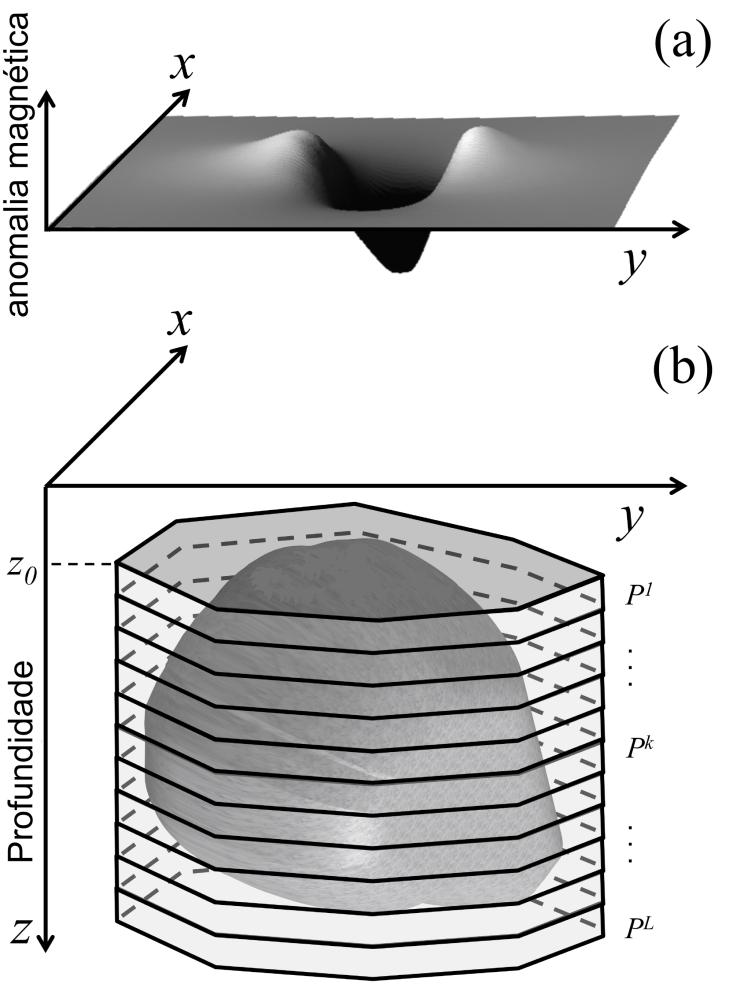
\includegraphics[scale=0.3]{figures/observed_data.png}
    \caption{Schematic representation of (a) total-filed anomaly (gray surface) produced by (b) a 3-D anomalous source (dark gray volume). The interpretation model in (b) consists of a set of L vertical, juxtaposed 3-D prisms $P^k$ , $k = 1,\dots, L$, (light gray prisms) in the vertical direction of a right-handed coordinate system.}
    \label{fig:obs}
\end{figure}

\begin{figure}
    \centering
    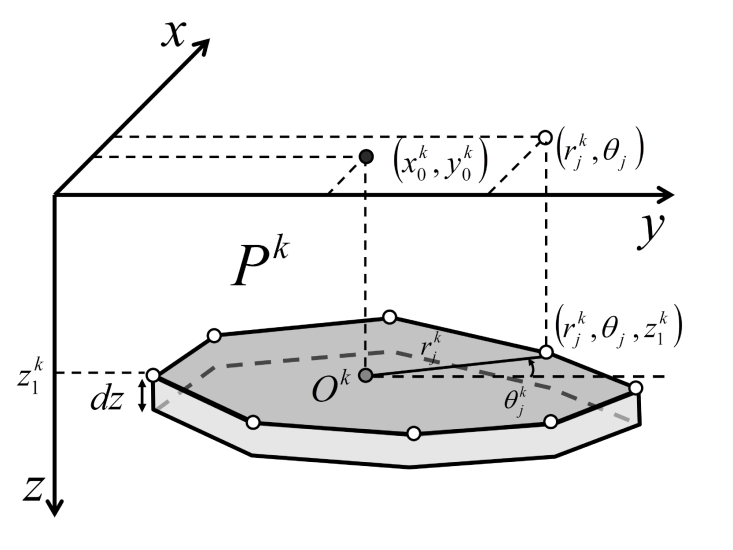
\includegraphics[scale=0.3]{figures/prism_parameters_mod.png}
    \caption{Polygonal cross-section of the $k$th vertical prism $P^k$ described by $V$ vertices (white dots) with polar coordinates ($r^k_j$ , $\theta ^k_j$), $j = 1, \dots, V$, $k = 1, \dots, L$ , referred to an arbitrary origin $O^k$ (grey dot) with horizontal Cartesian coordinates ($x_0^k$ , $y_0^k$), $k = 1, \dots, L$ , (black dot).}
    \label{fig:prism_parameters}
\end{figure}

\begin{figure}
    \centering
    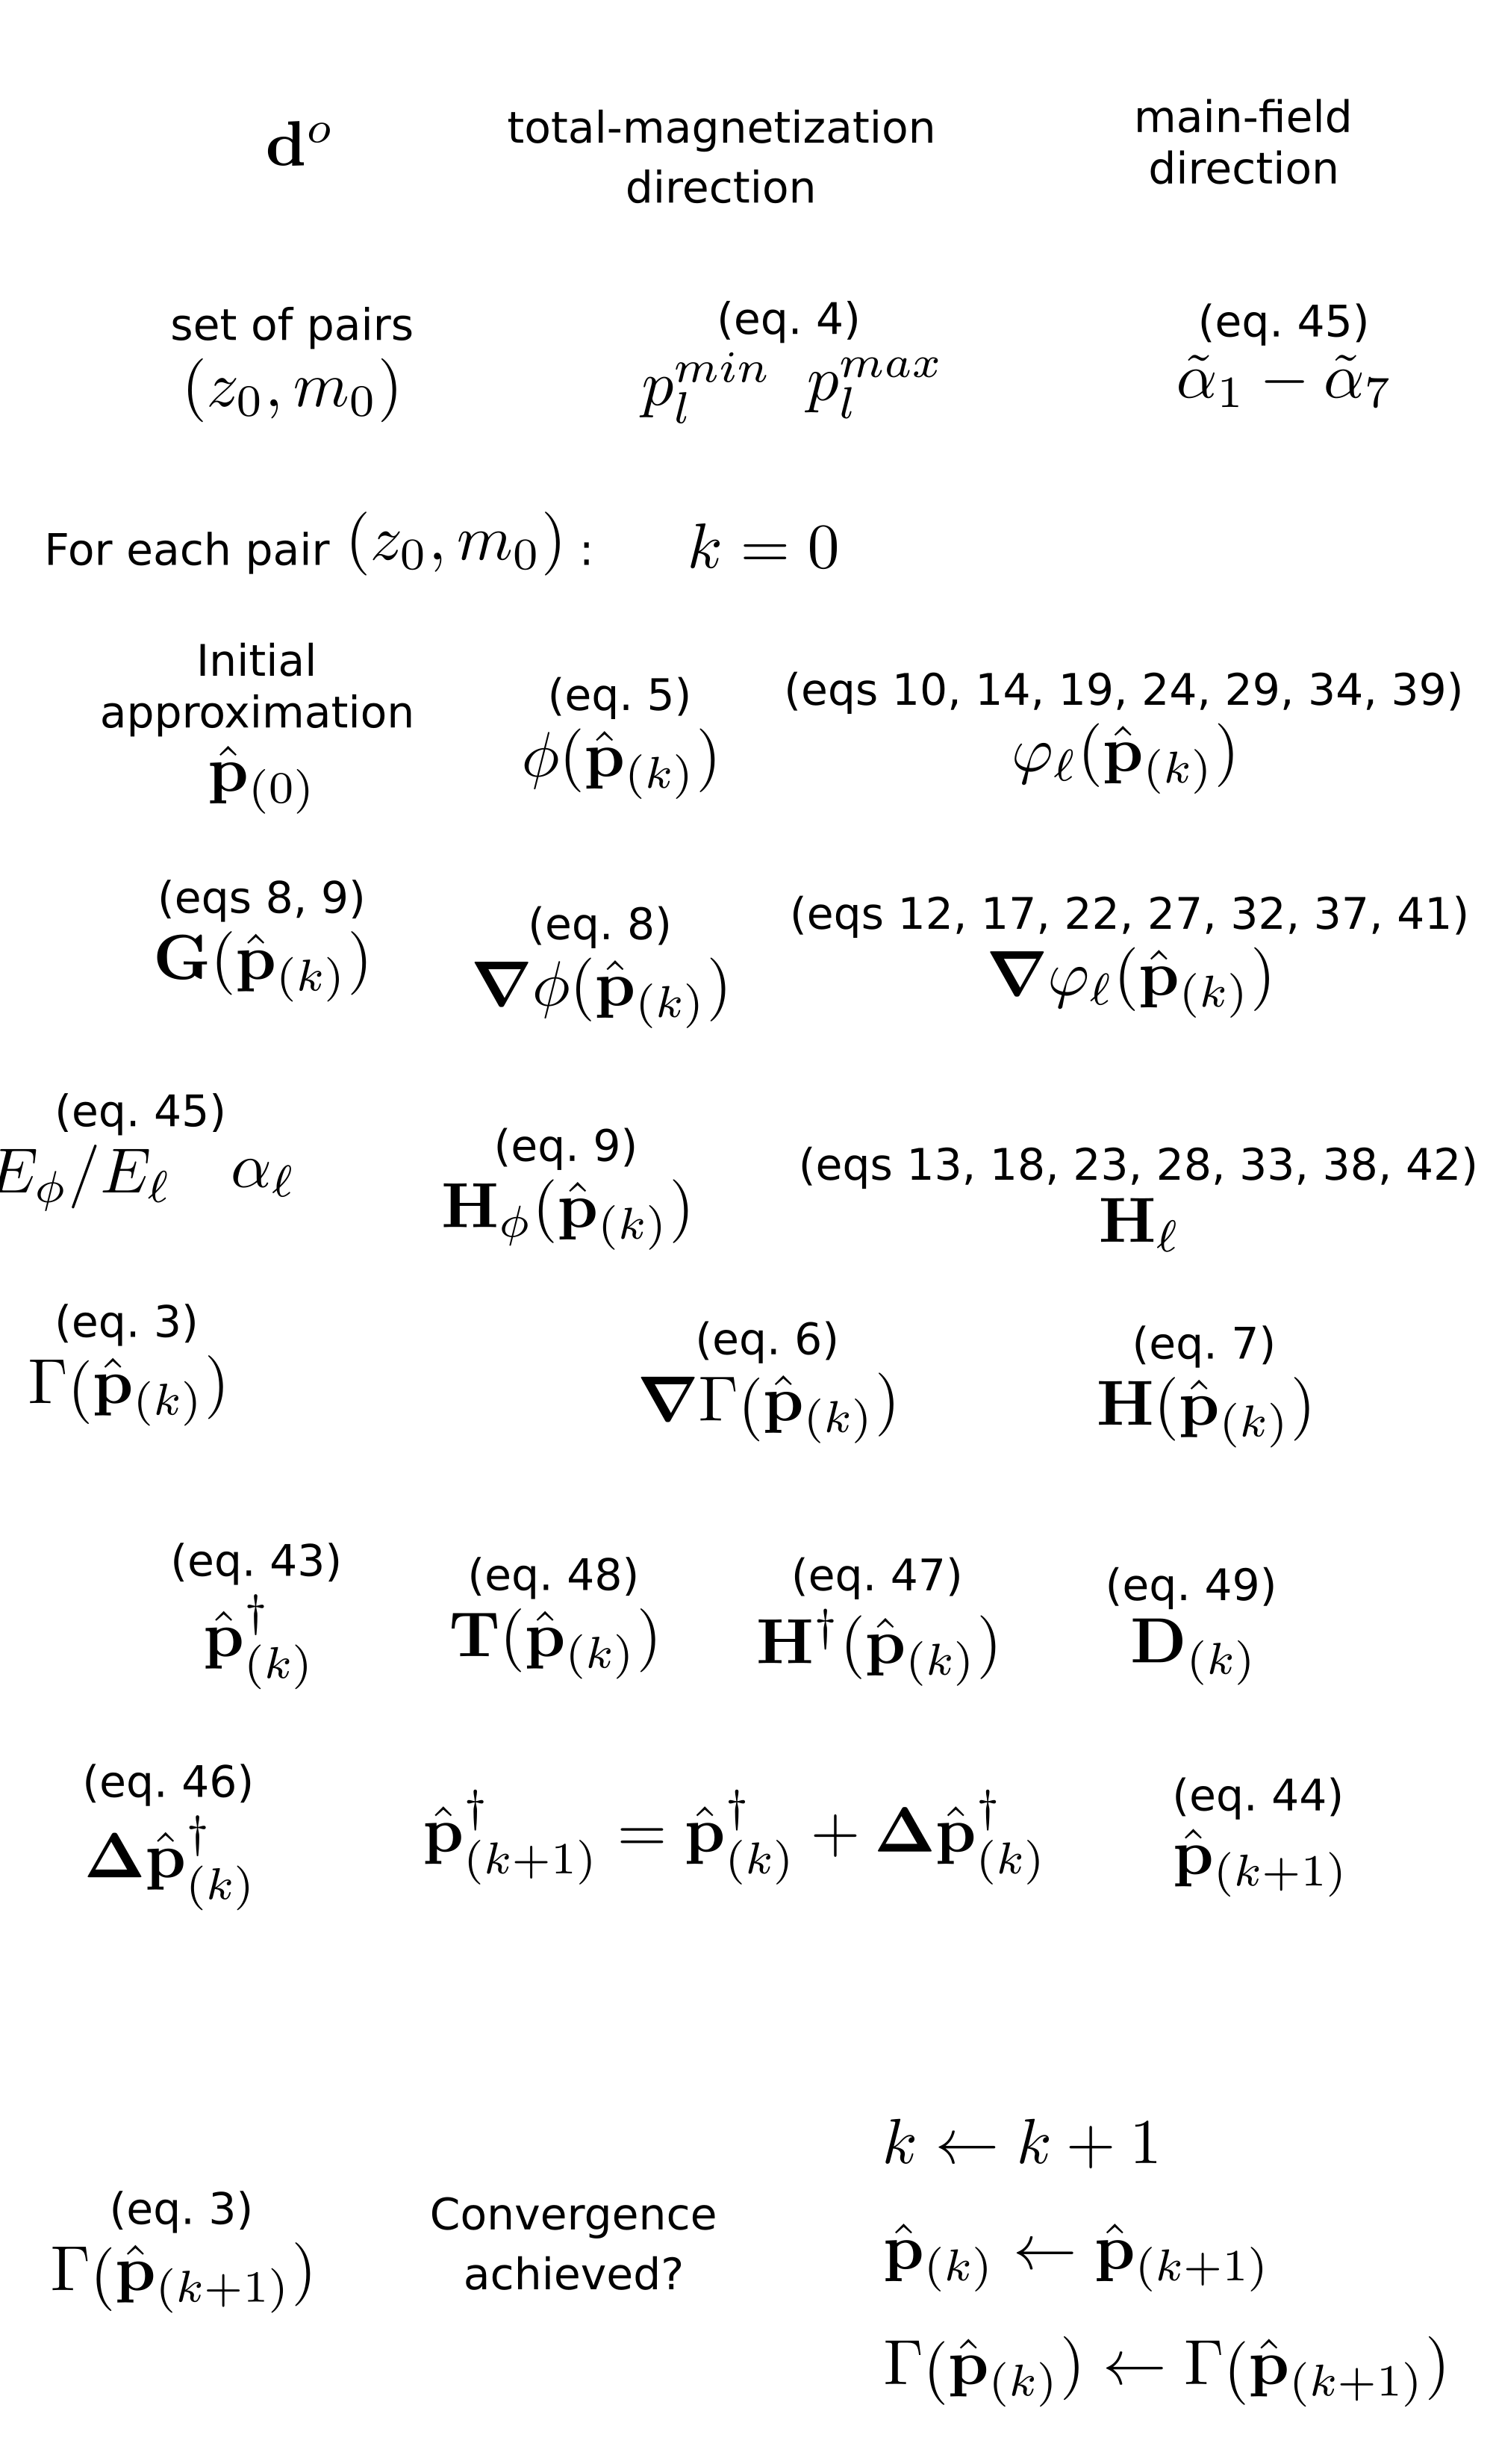
\includegraphics[scale=0.8]{figures/flowchart.png}
    \caption{Flowchart of our algorithm.}
    \label{fig:flowchart}
\end{figure}

% Application to synthetic data - simple model

\begin{figure}
    \centering
    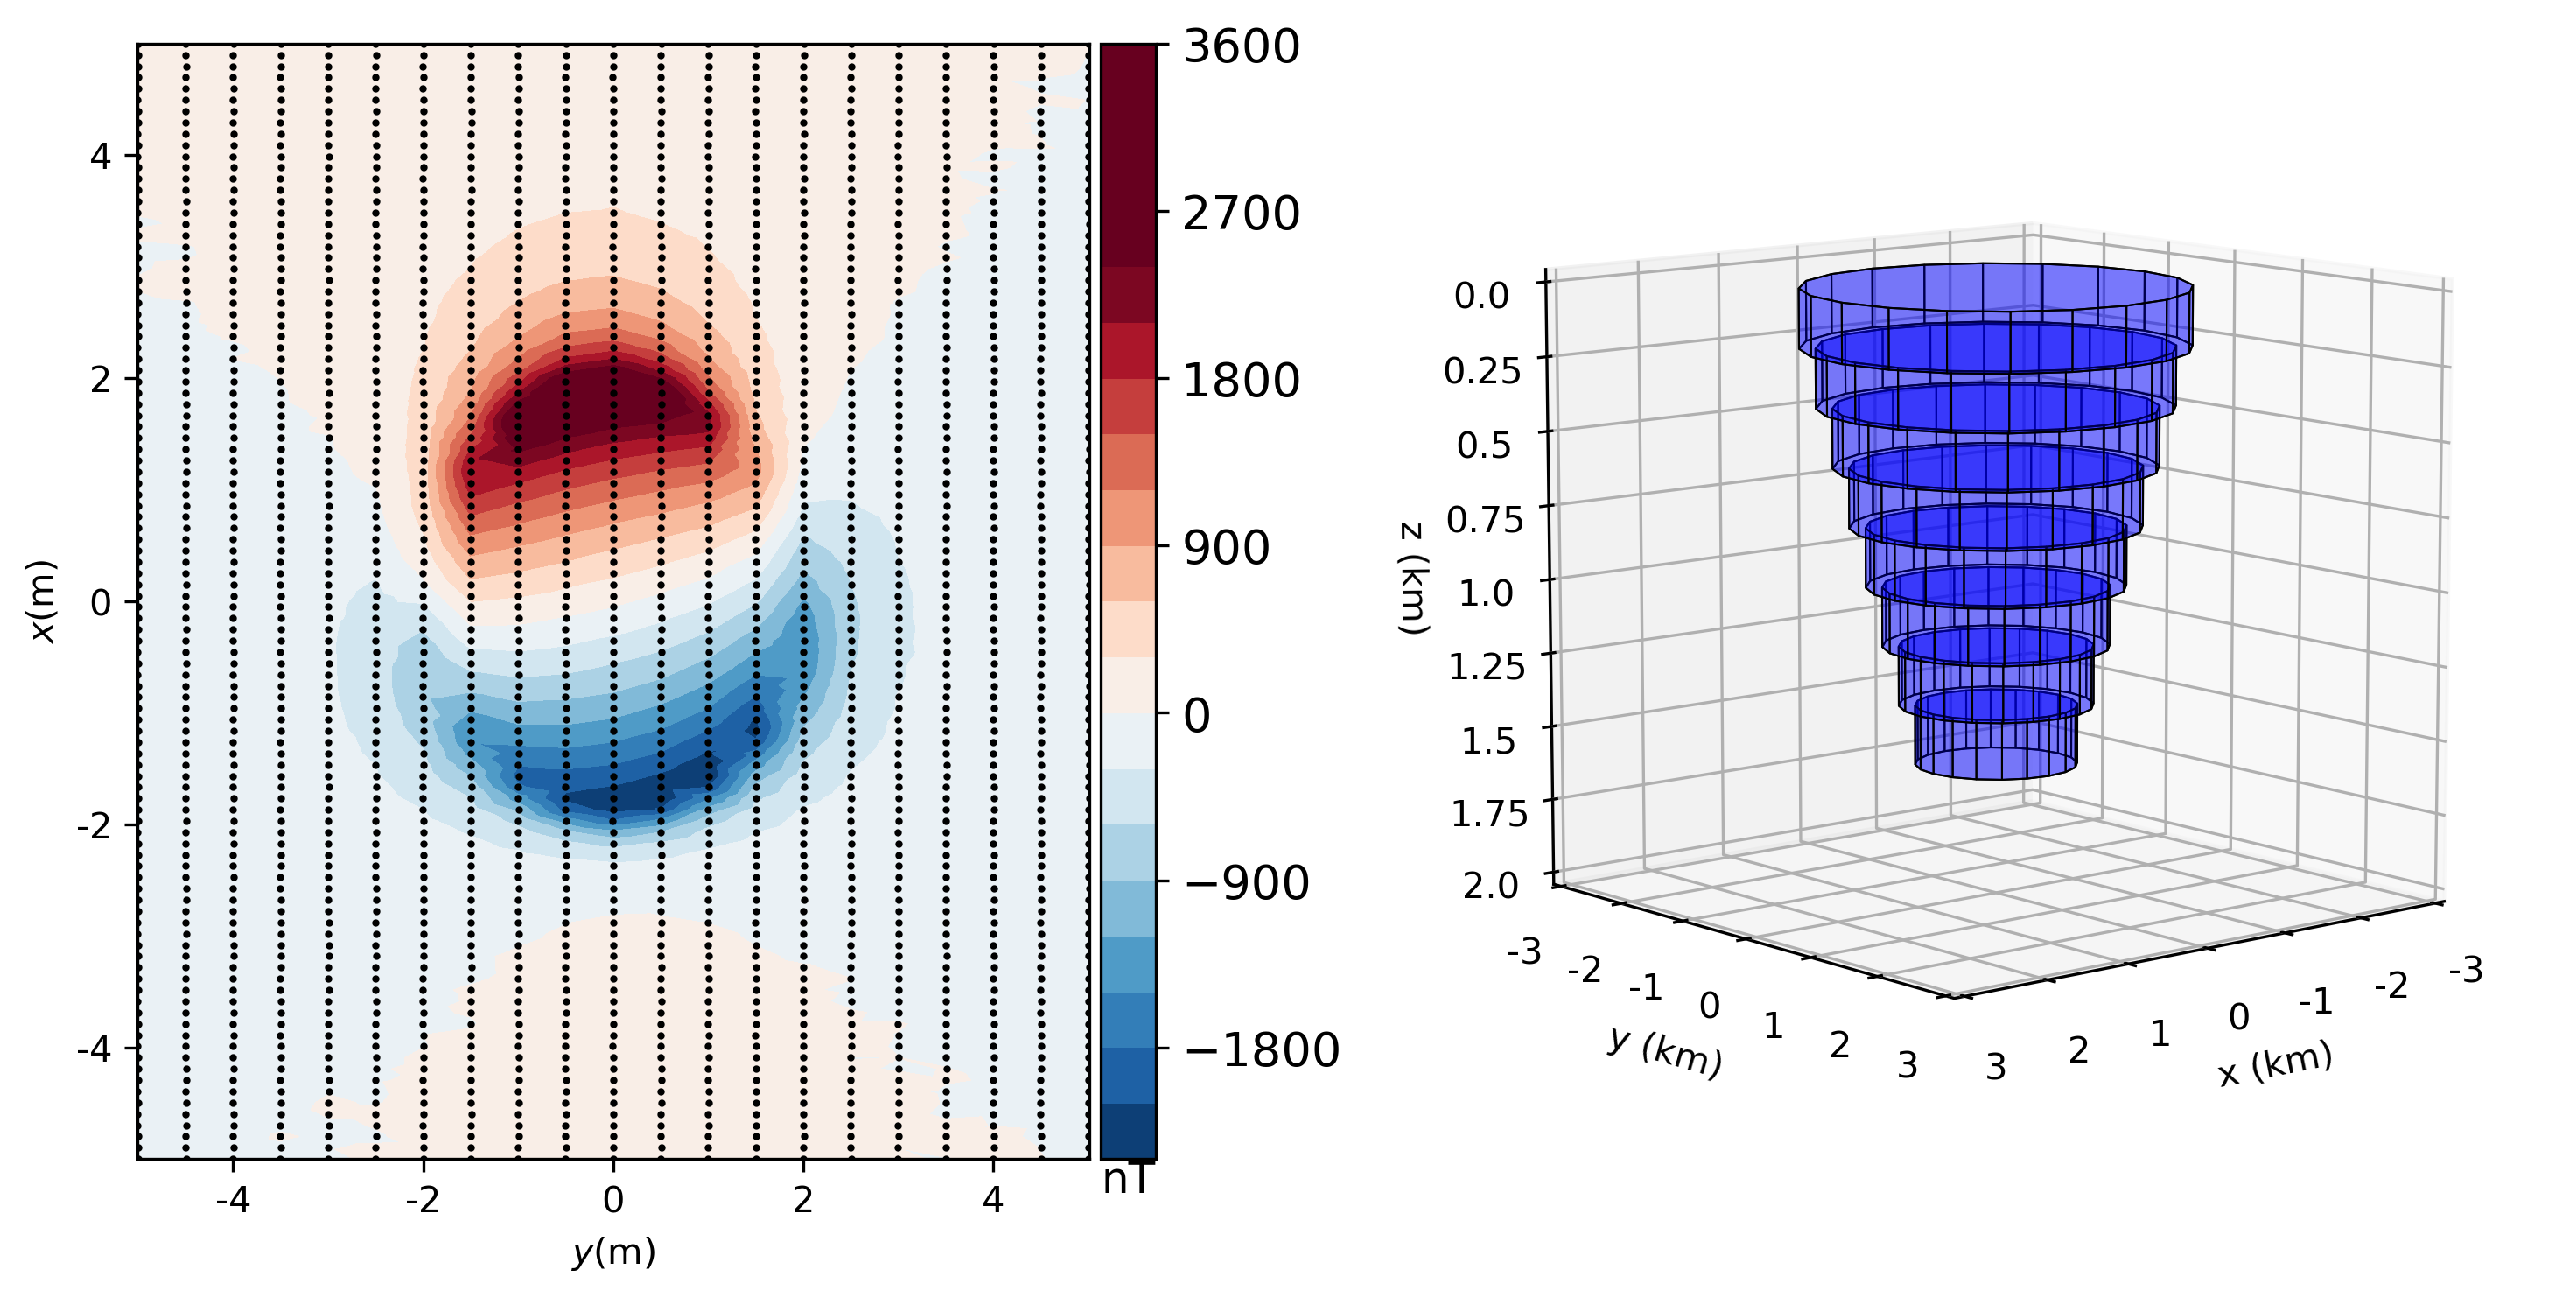
\includegraphics[scale=.5]{figures/wedding_cake_model_data.png}
    \caption{Simple model simulation. (a) noise-corrupted total-field anomaly produced by the simple model (blue prisms) in (b). The black dots represent the observation points simulating an airborne survey.
}
    \label{fig:kimb_model}
\end{figure}

\begin{figure}
	\centering
	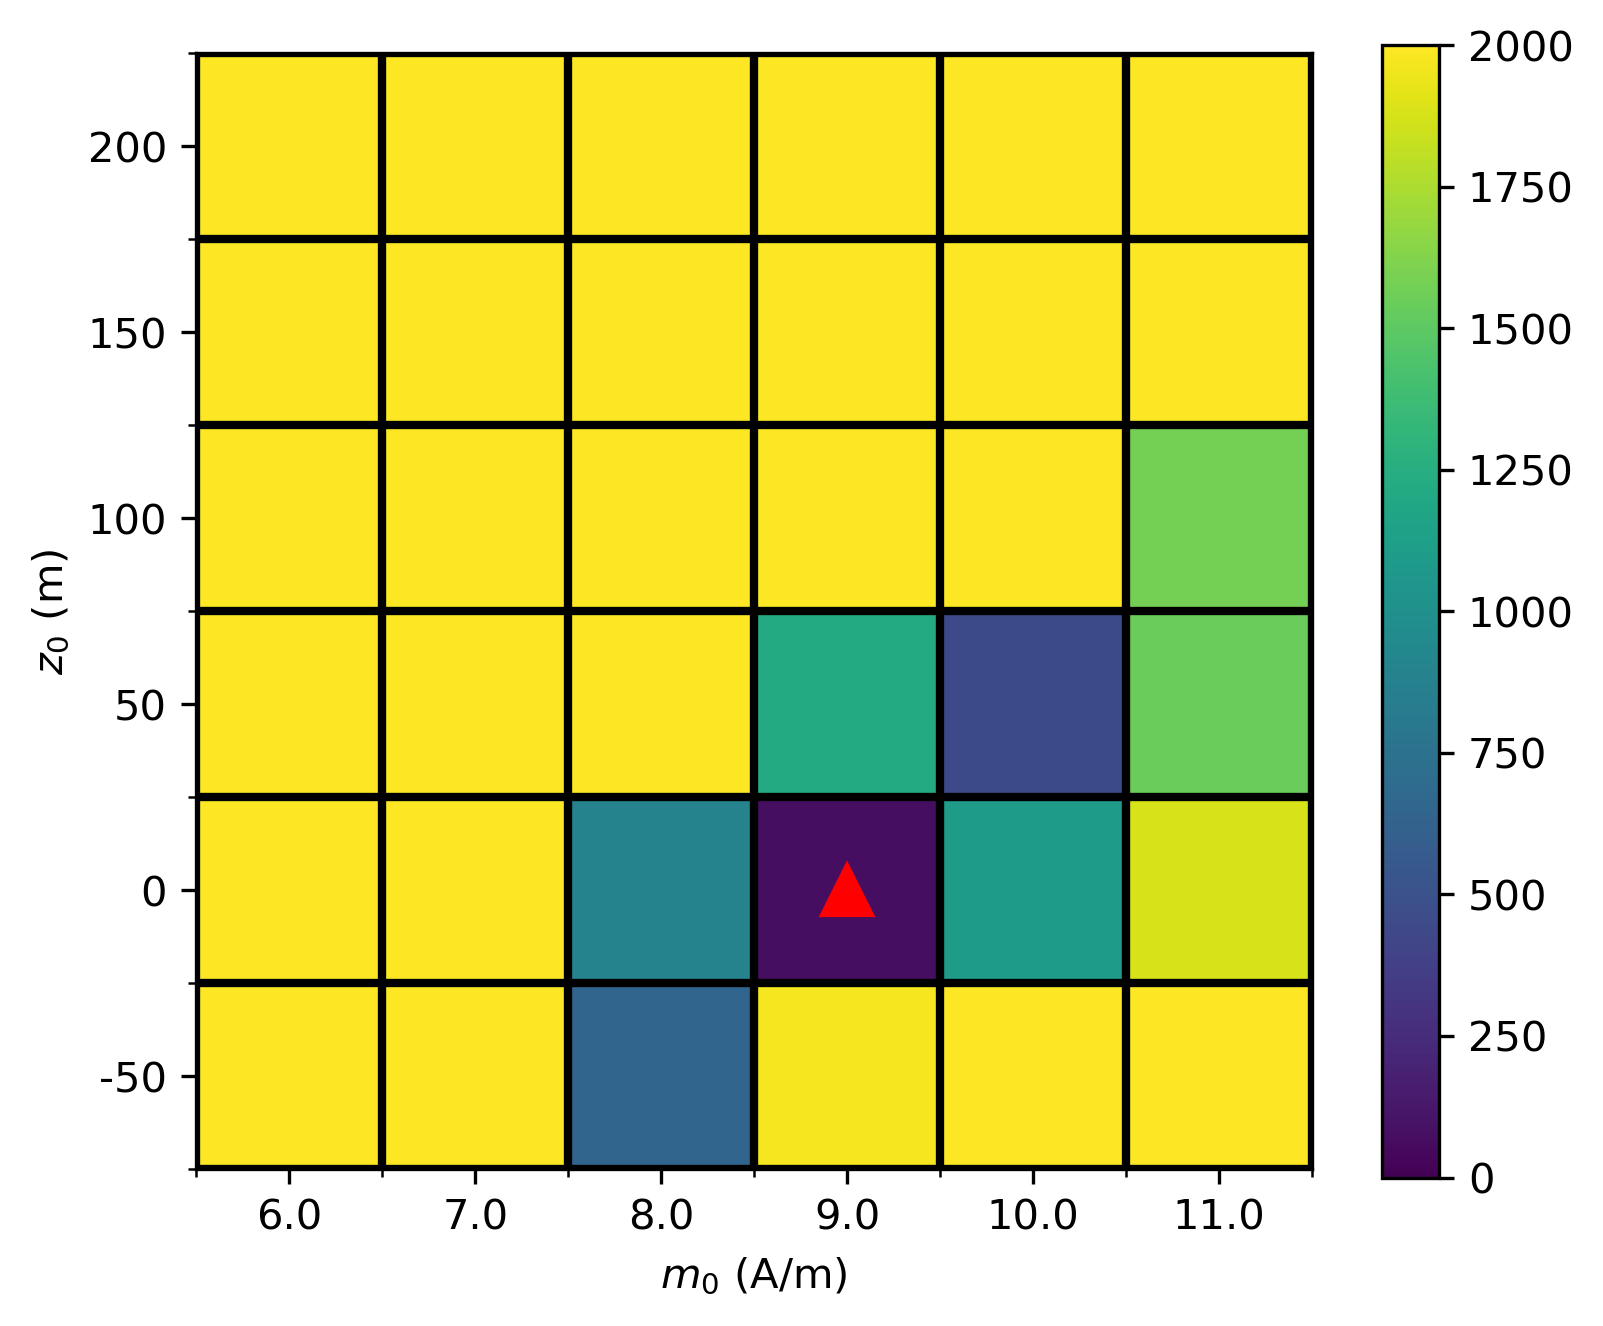
\includegraphics[scale=.75]{figures/wedding_cake_obj_func_map.png}
	\caption{Map of the objective function values due to the inverse solutions for the simple model. The range of $m_0$ varies from $6$ to $11$ A/m in a step of $1$ A/m and the range of $z_0$ varies from $-50$ to $200$ m in a step of $50$ m. Each square is a value of the goal function (eq. \ref{eq:gamma}) of a solution of the inverse problem for a pair of the total-magnetization intensity and the depth to the top of the source. The red triangle represents the true values for $m_0 = 9$ A/m and $z_0=0$m.
	}
	\label{fig:kimb_map}
\end{figure}

\begin{figure}
	\centering
	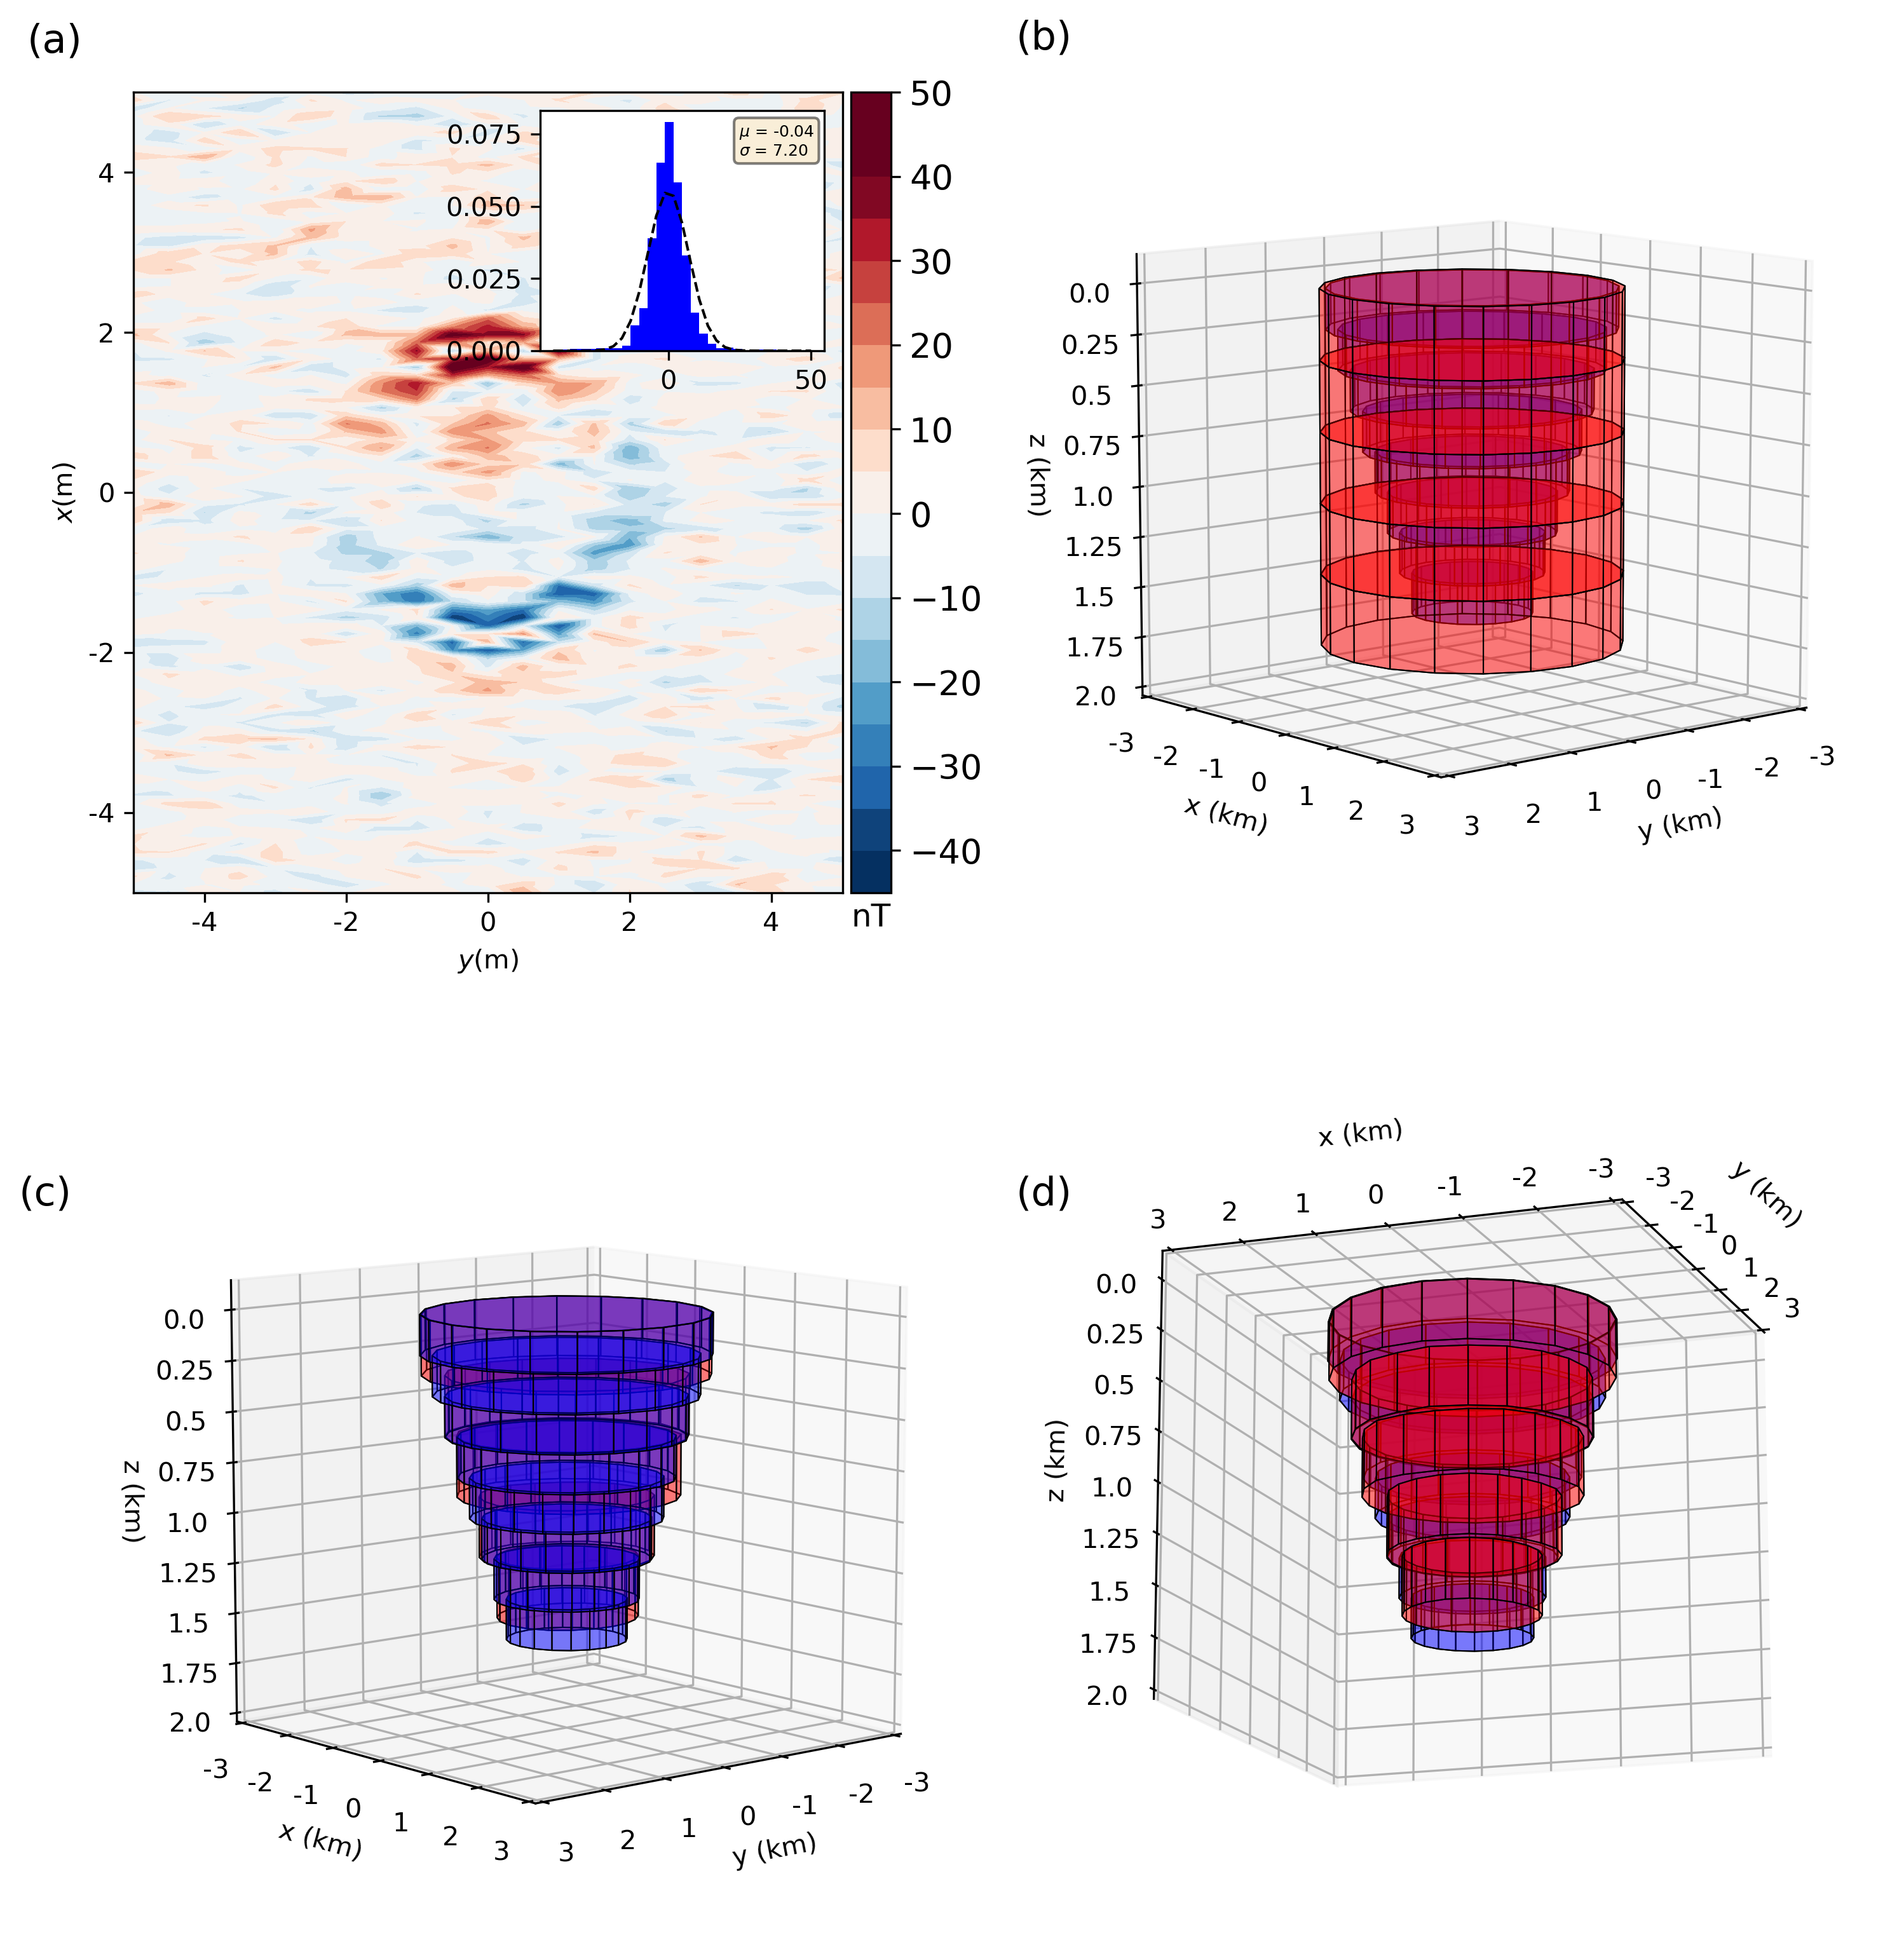
\includegraphics[scale=.5]{figures/wedding_cake_results.png}
	\caption{Application to simple model data. (a) residual data given by the difference between the noise-corrupted data (Fig. \ref{fig:kimb_model}a) and the predicted data (not shown) produced by the estimated model (red prisms) in (c) and (d). These inversions were computed using the same cylinder as a initial approximation. The red prisms in (b) represent the initial approximate of the inversion.
	}
	\label{fig:kimb_results}
\end{figure}

% Application to synthetic data - complex model

\begin{figure}
    \centering
    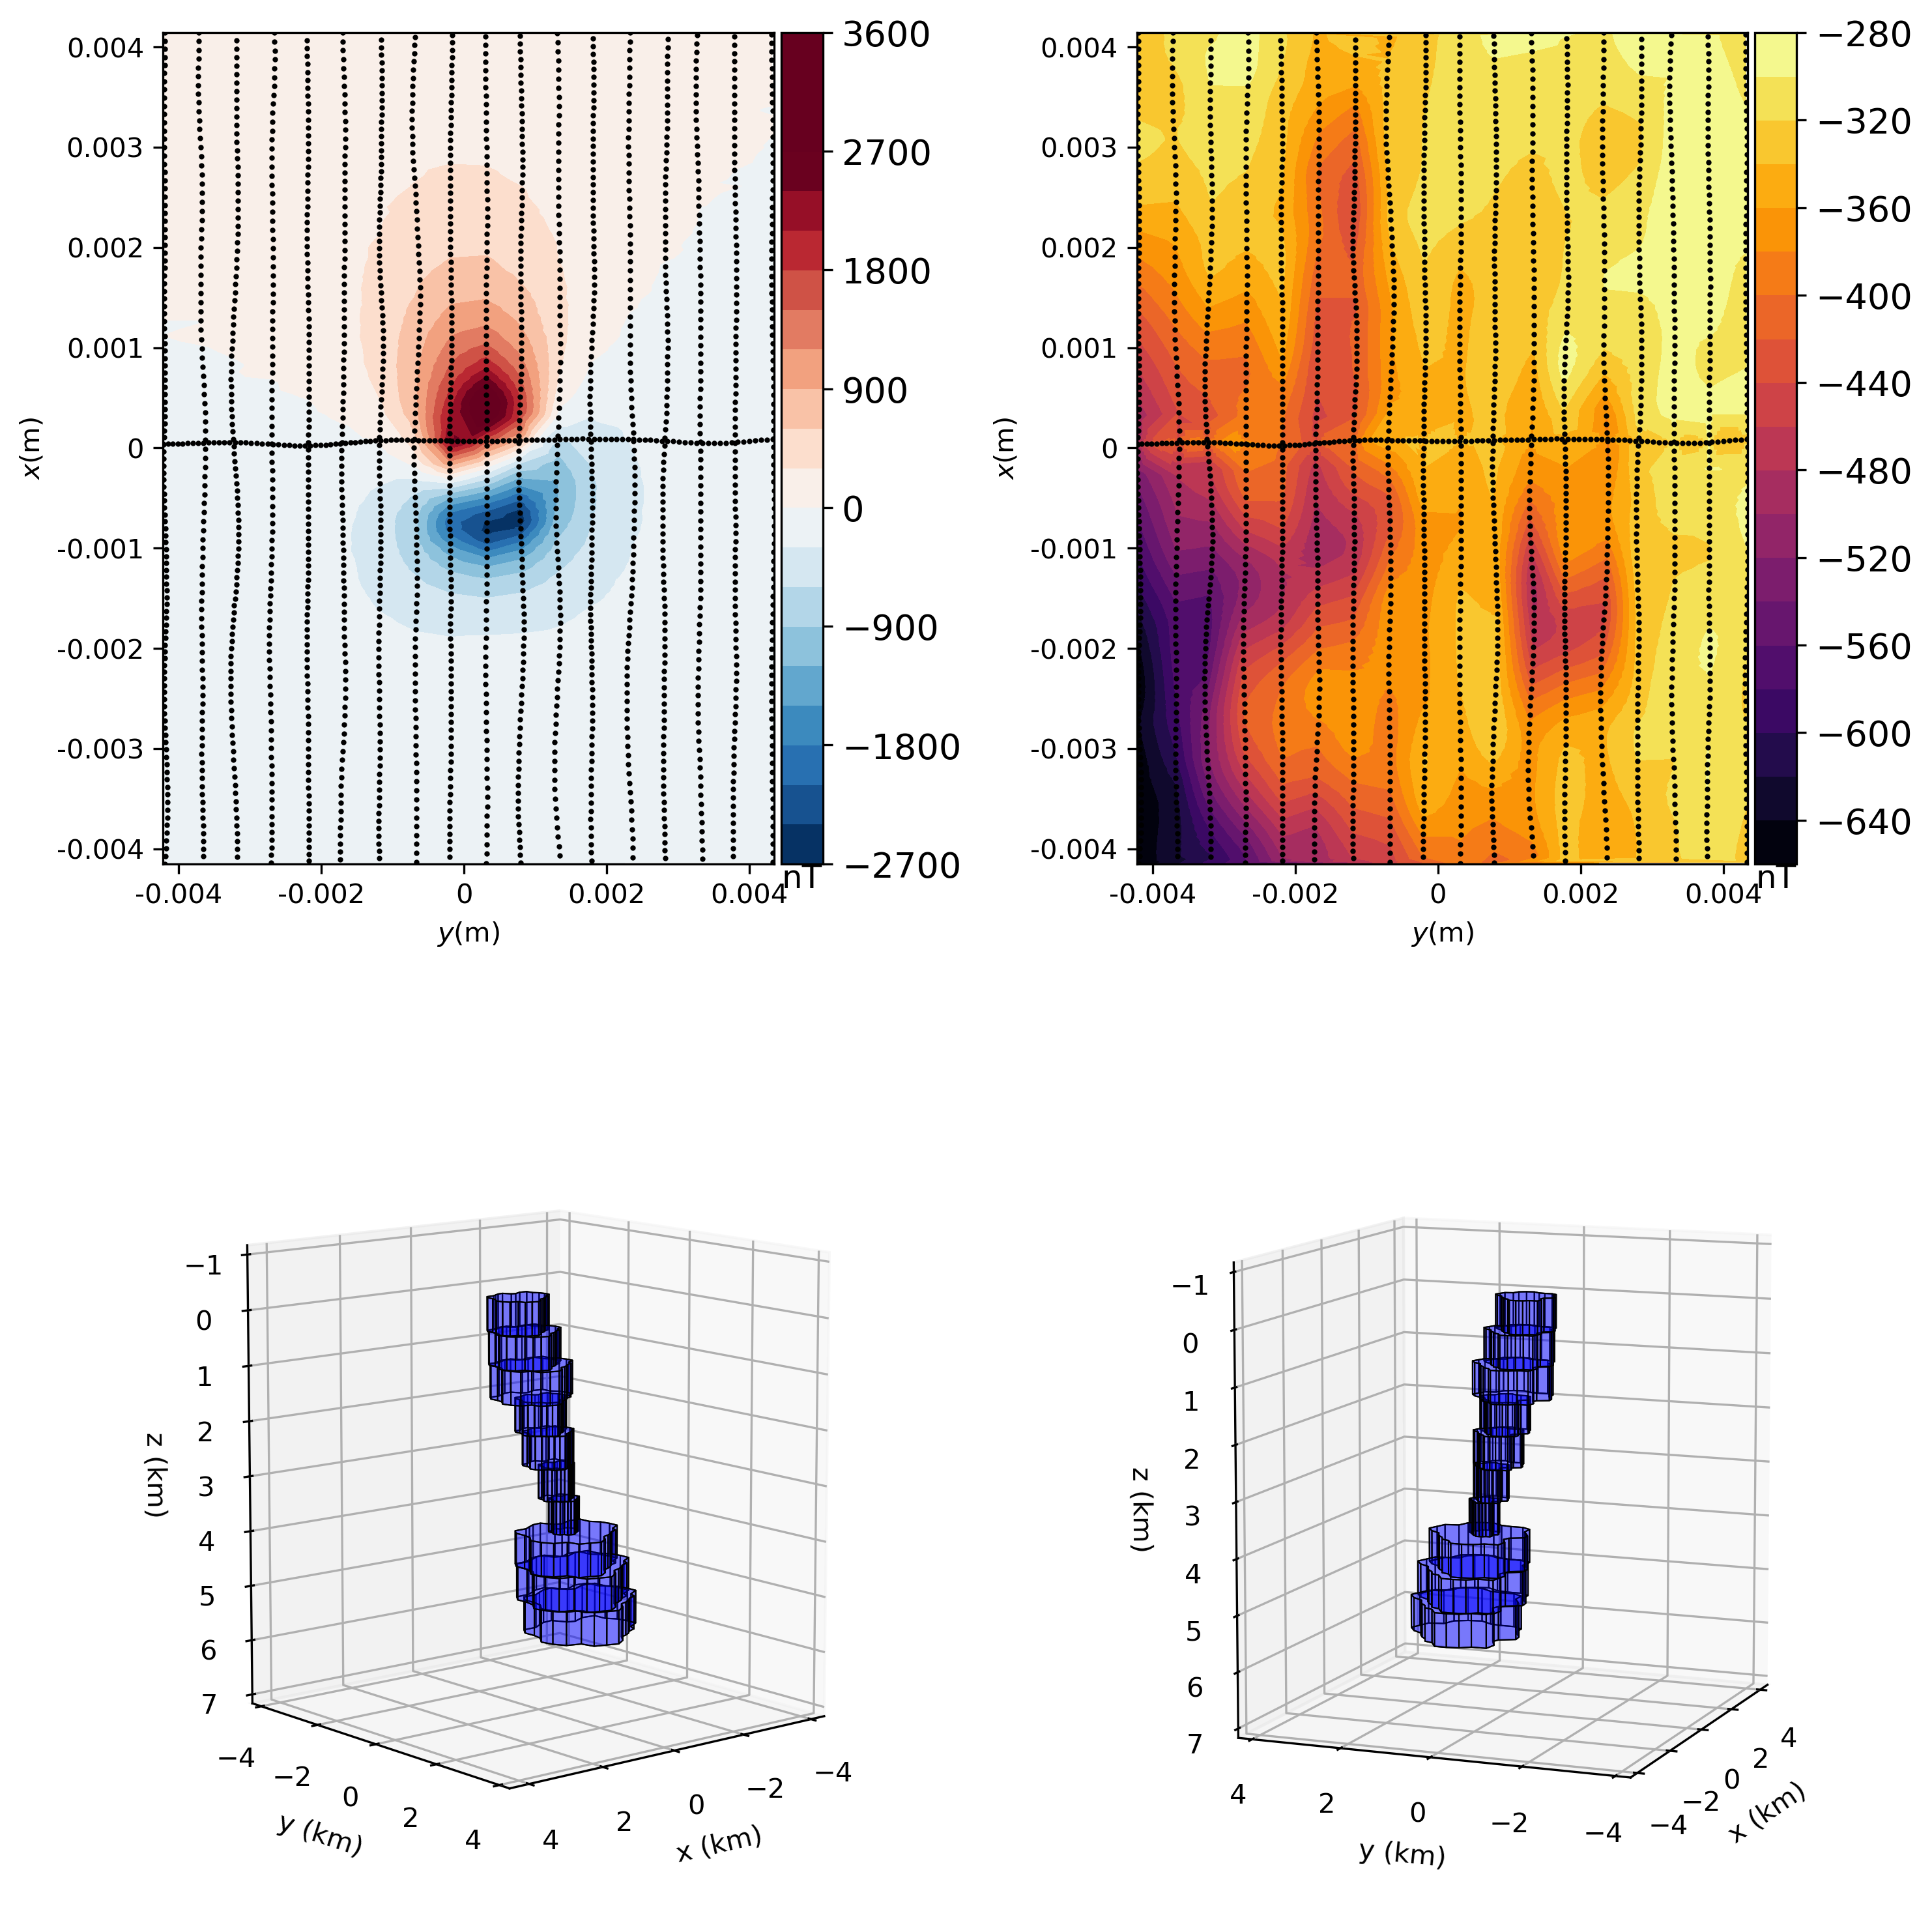
\includegraphics[scale=.5]{figures/complex_model_data.png}
    \caption{Complex model simulation. (a) noise-corrupted total-field anomaly, the black dots represent the observation points. (b) elevation of the observations simulating an airborne survey produced by the complex model (blue prisms) in (c) and (d).
}
    \label{fig:complex_model}
\end{figure}

\begin{figure}
	\centering
	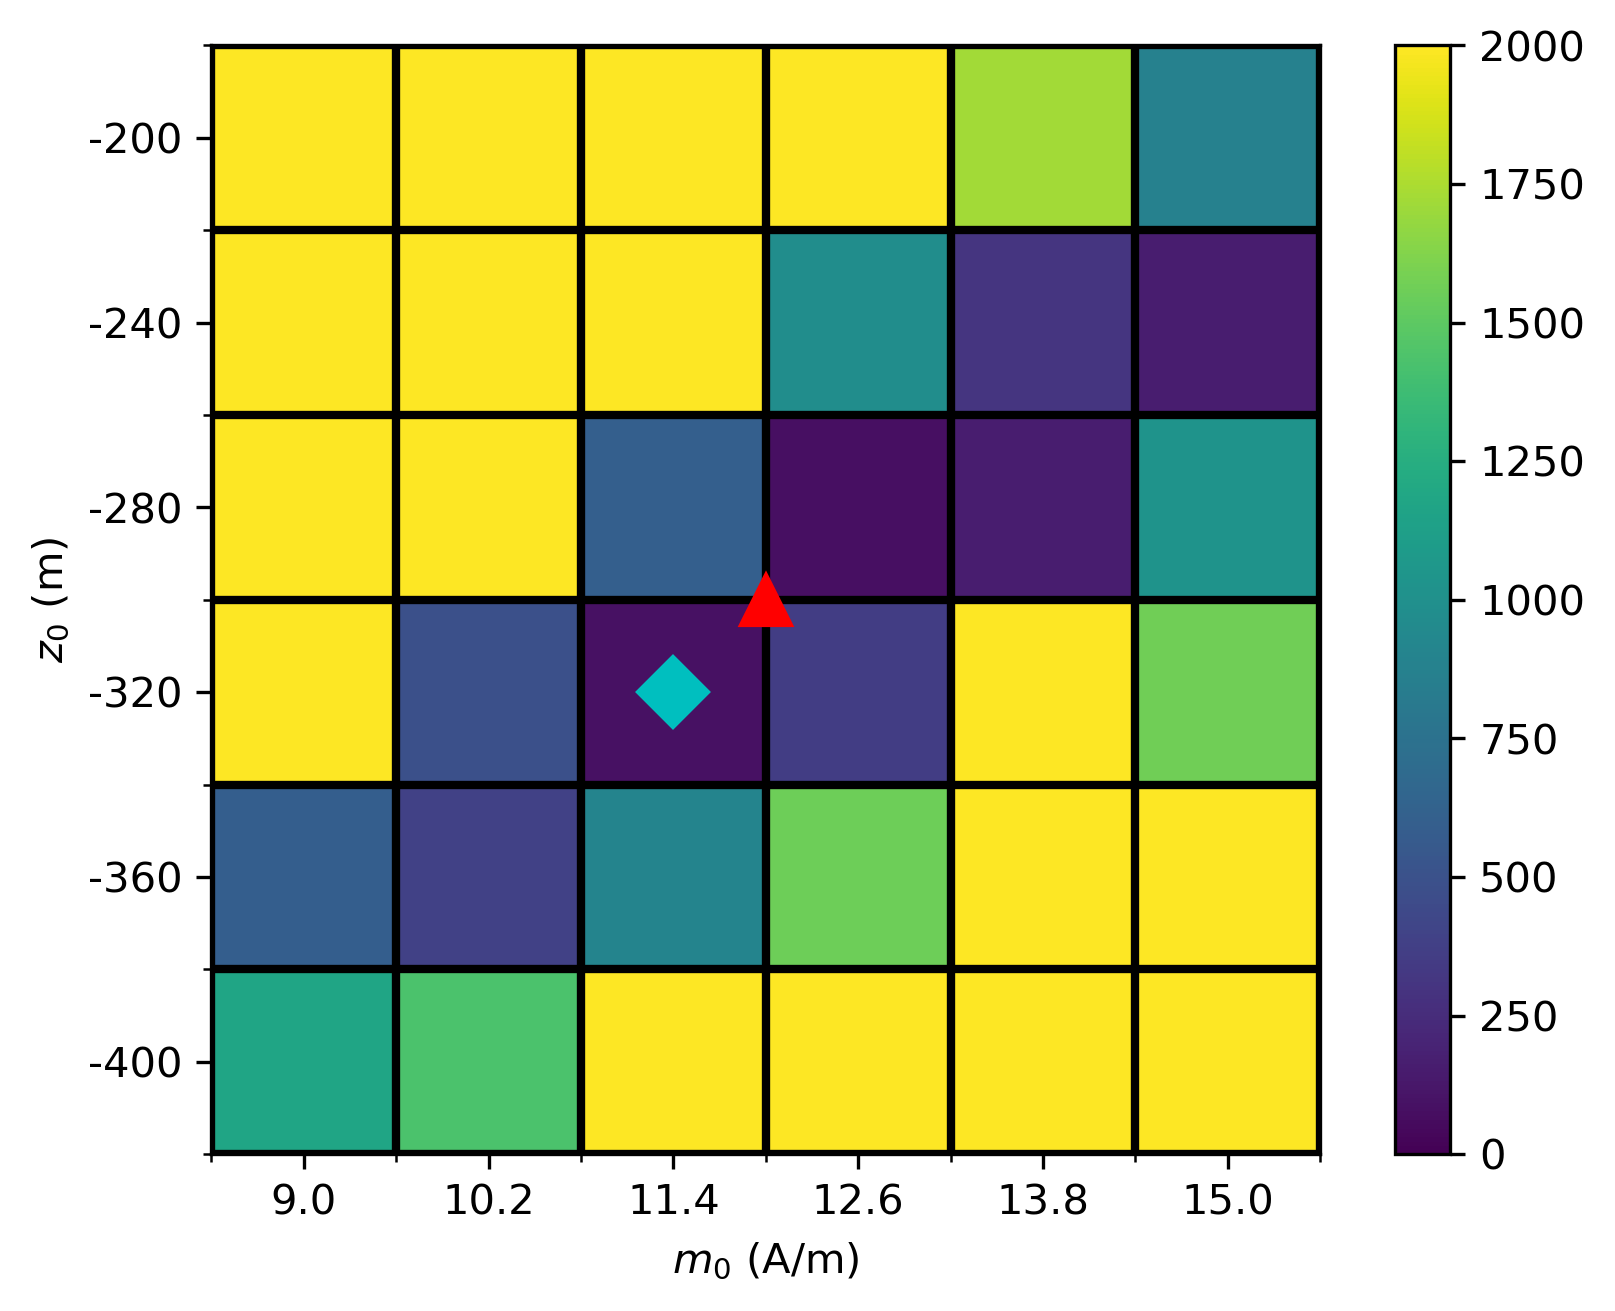
\includegraphics[scale=.75]{figures/complex_obj_func_map.png}
	\caption{Map of the objective function values due to the inverse solutions for the complex model. The range of $m_0$ varies from $9$ to $15$ A/m in a step of $1.2$ A/m and the range of $z_0$ varies from $-400$ to $-200$ m in a step of $50$ m. Each square is a value of the goal function (eq. \ref{eq:gamma}) of a solution of the inverse problem for a pair of the total-magnetization intensity and the depth to the top of the source. These inversions were computed using the same cylinder as a initial approximation. The red triangle represents the true values for $m_0$ and $z_0$. The cyan diamond represents the solution with the lowest function value.
	}
	\label{fig:complex_map}
\end{figure}

\begin{figure}
    \centering
    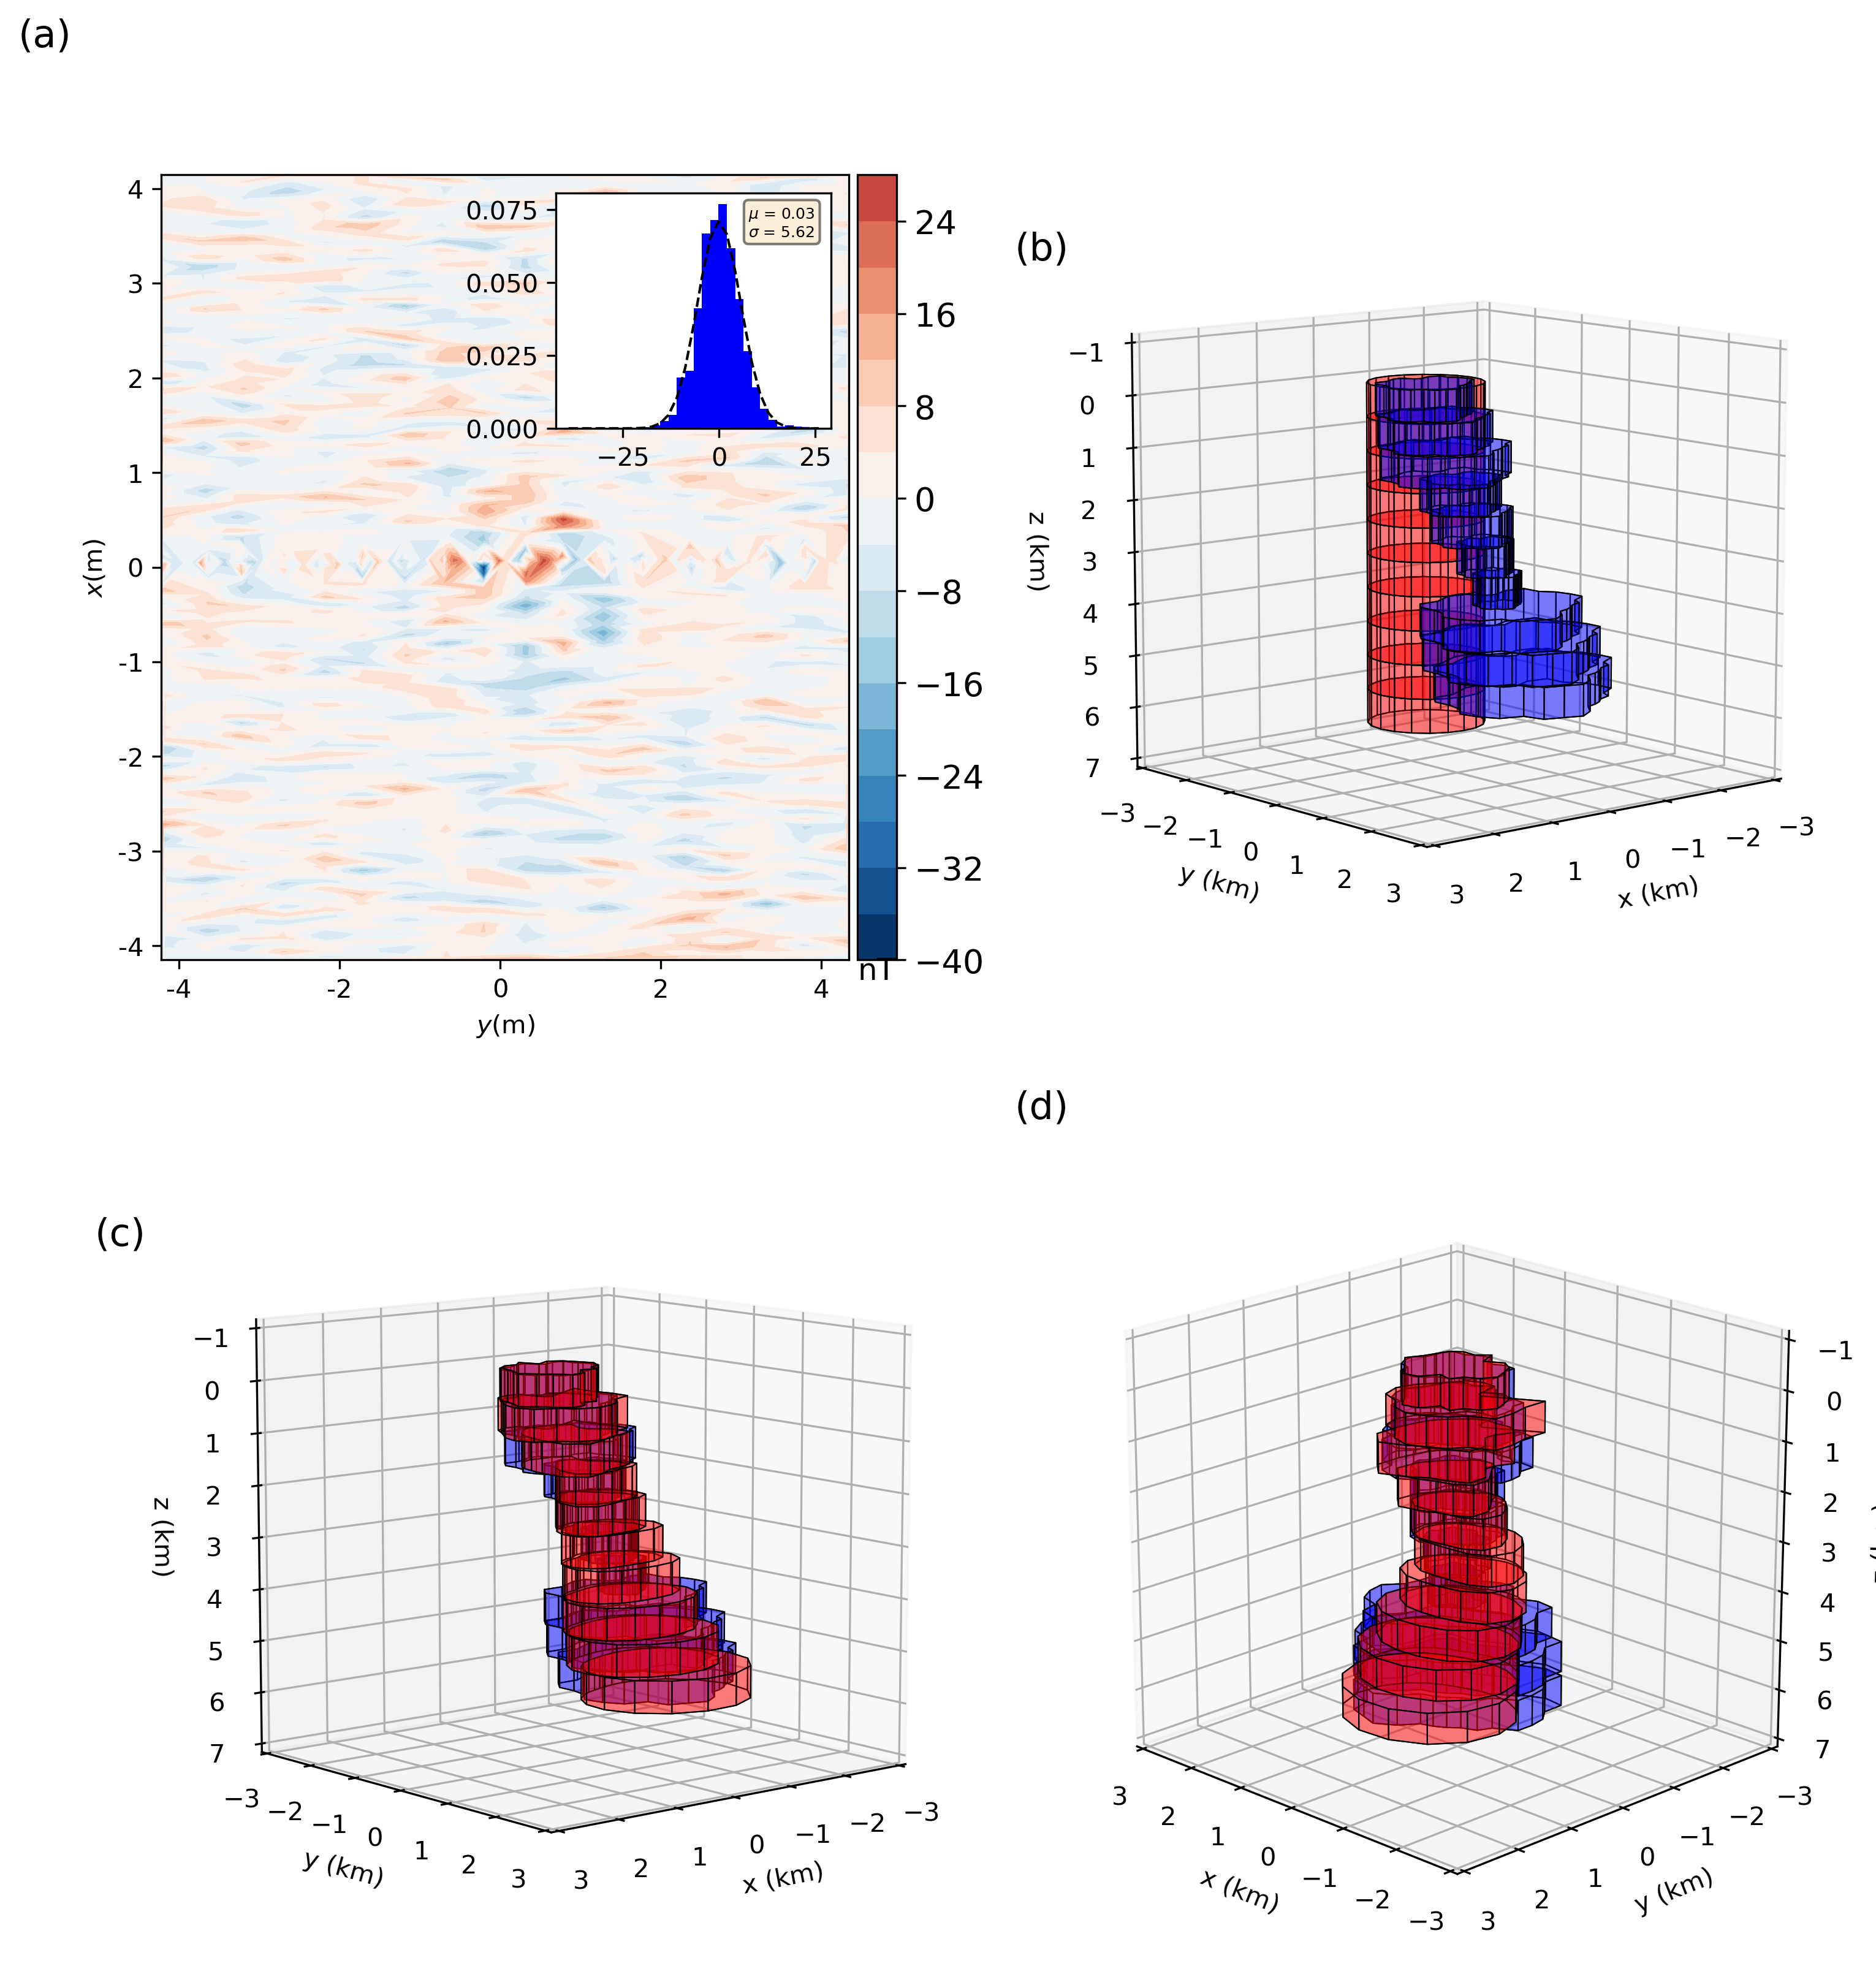
\includegraphics[scale=.5]{figures/complex_results.png}
    \caption{Application to complex model data. (a) residual data given by the difference between the noise-corrupted data (Fig. \ref{fig:complex_model}a) and the predicted data (not shown) produced by the estimated model (red prisms) in (c) and (d). The red prisms in (b) represent the initial approximate of the inversion.
}
    \label{fig:complex_result}
\end{figure}

% Application to field data

\begin{figure}
    \centering
    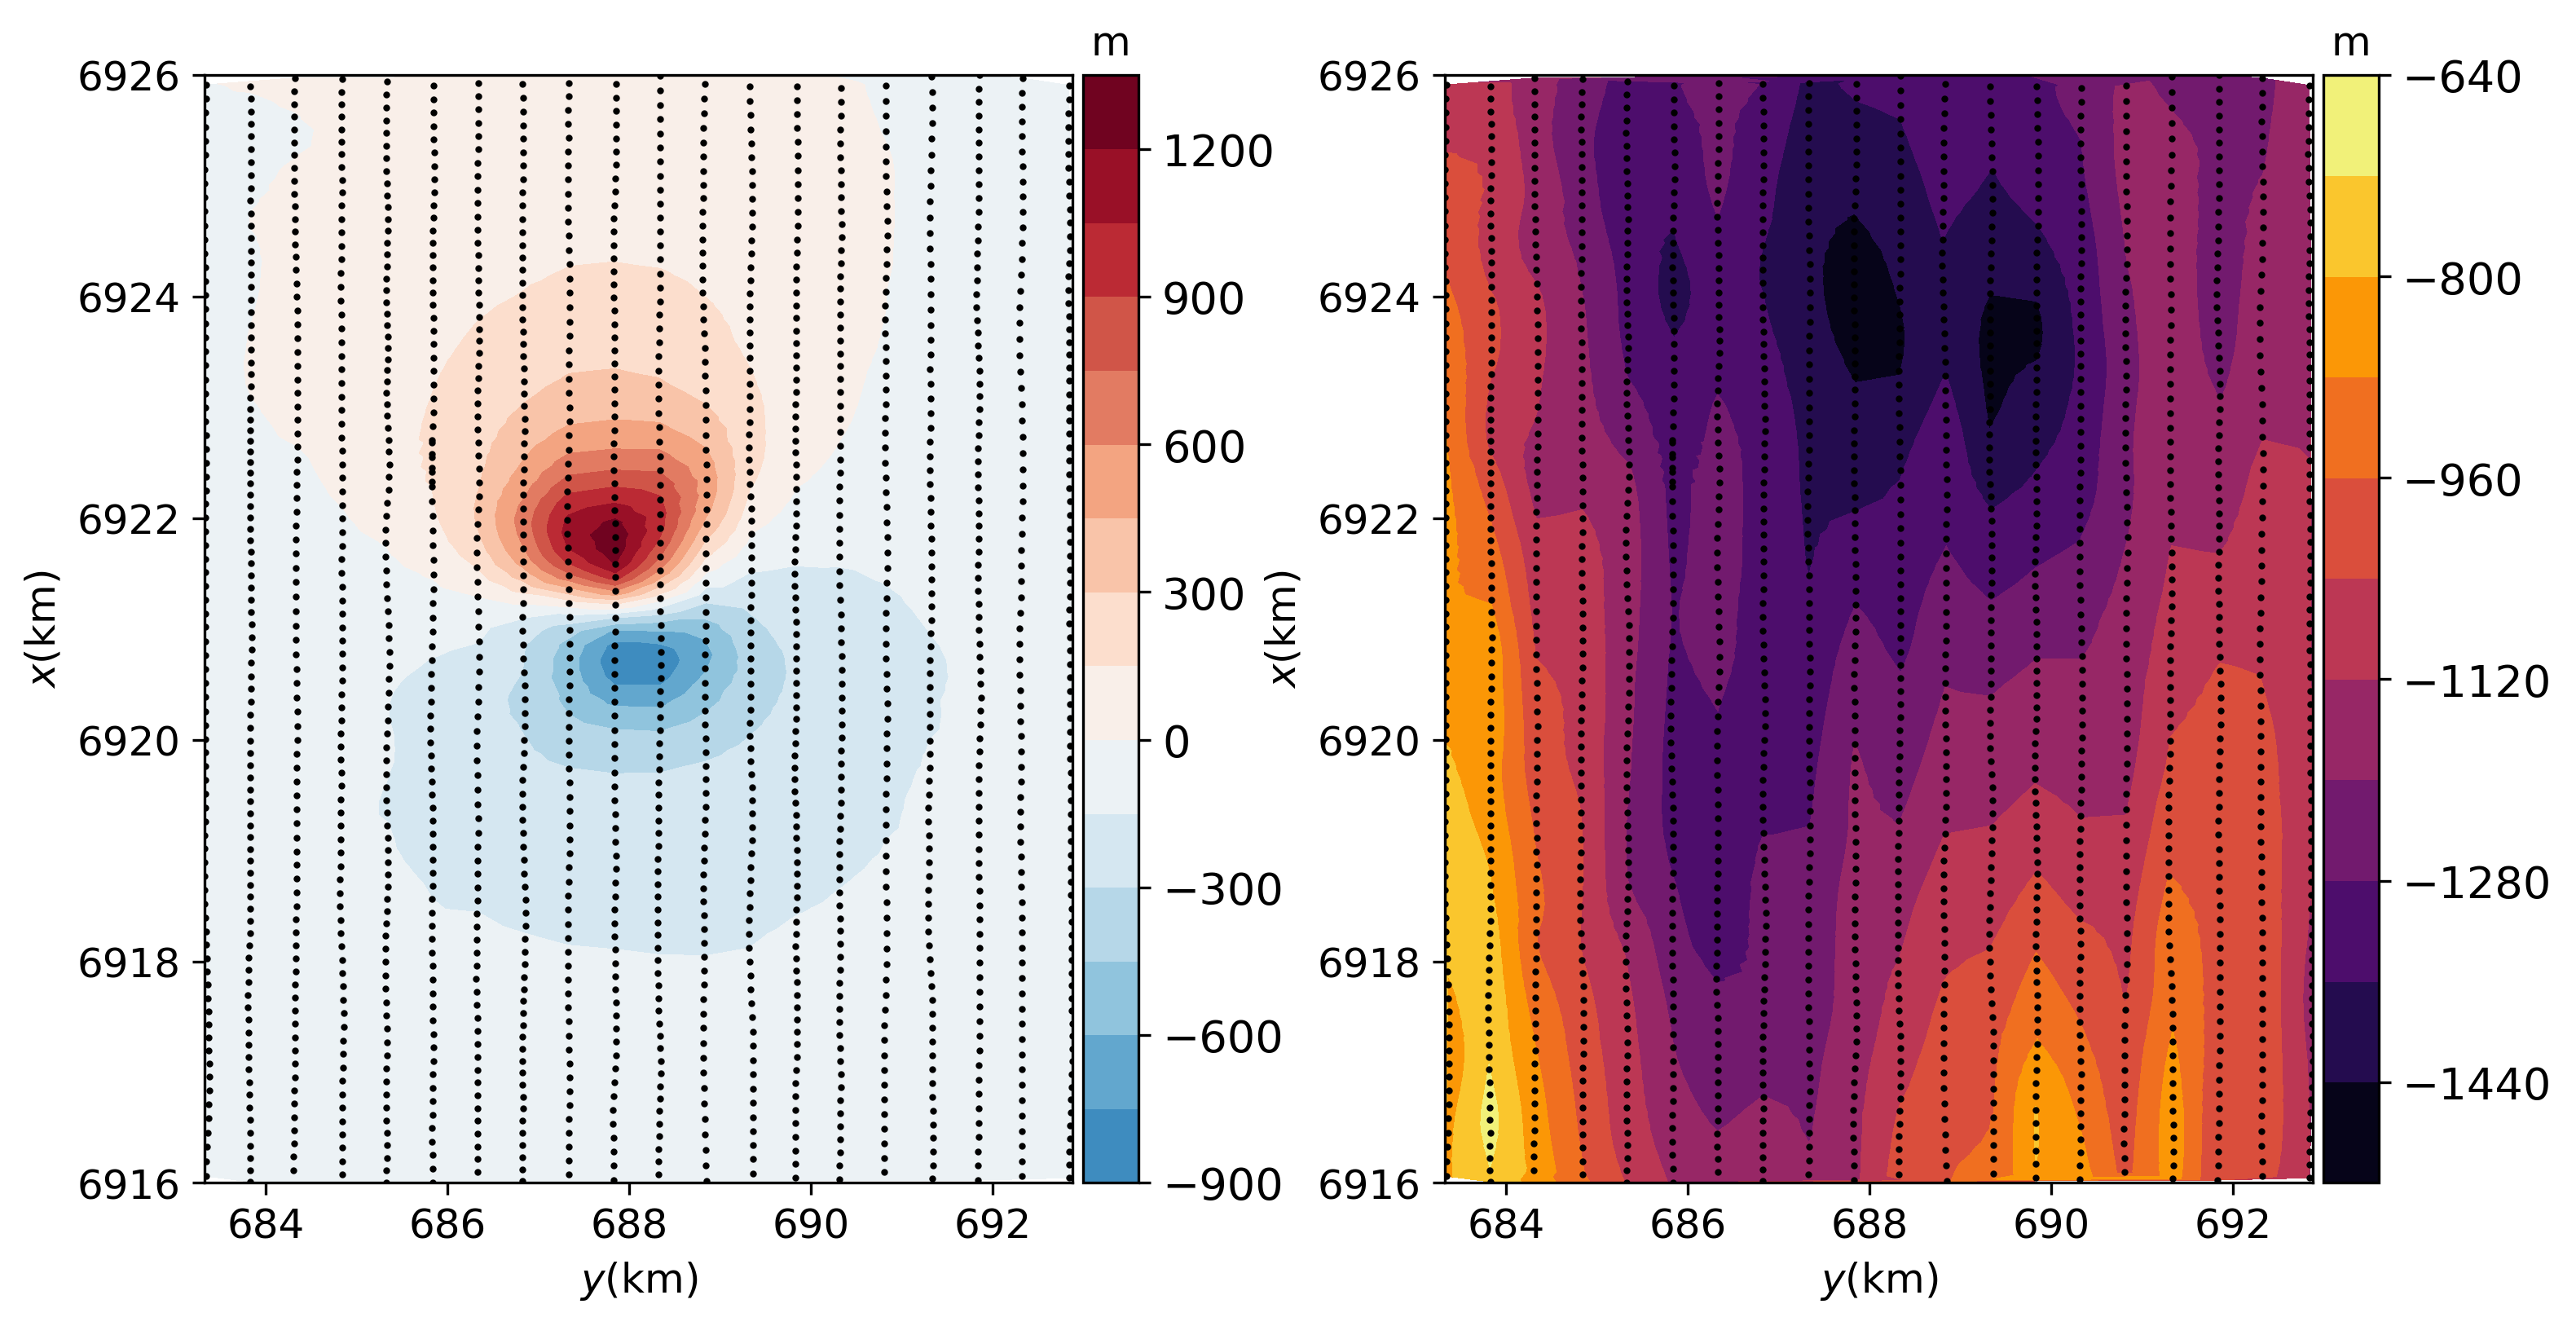
\includegraphics[scale=.5]{figures/anitapolis_data_alt.png}
    \caption{Field data application. (a) total-field anomaly of Anitapolis, the black dots are the observation points. (b) elevation of the observations.
}
    \label{fig:real_data}
\end{figure}

\begin{figure}
	\centering
	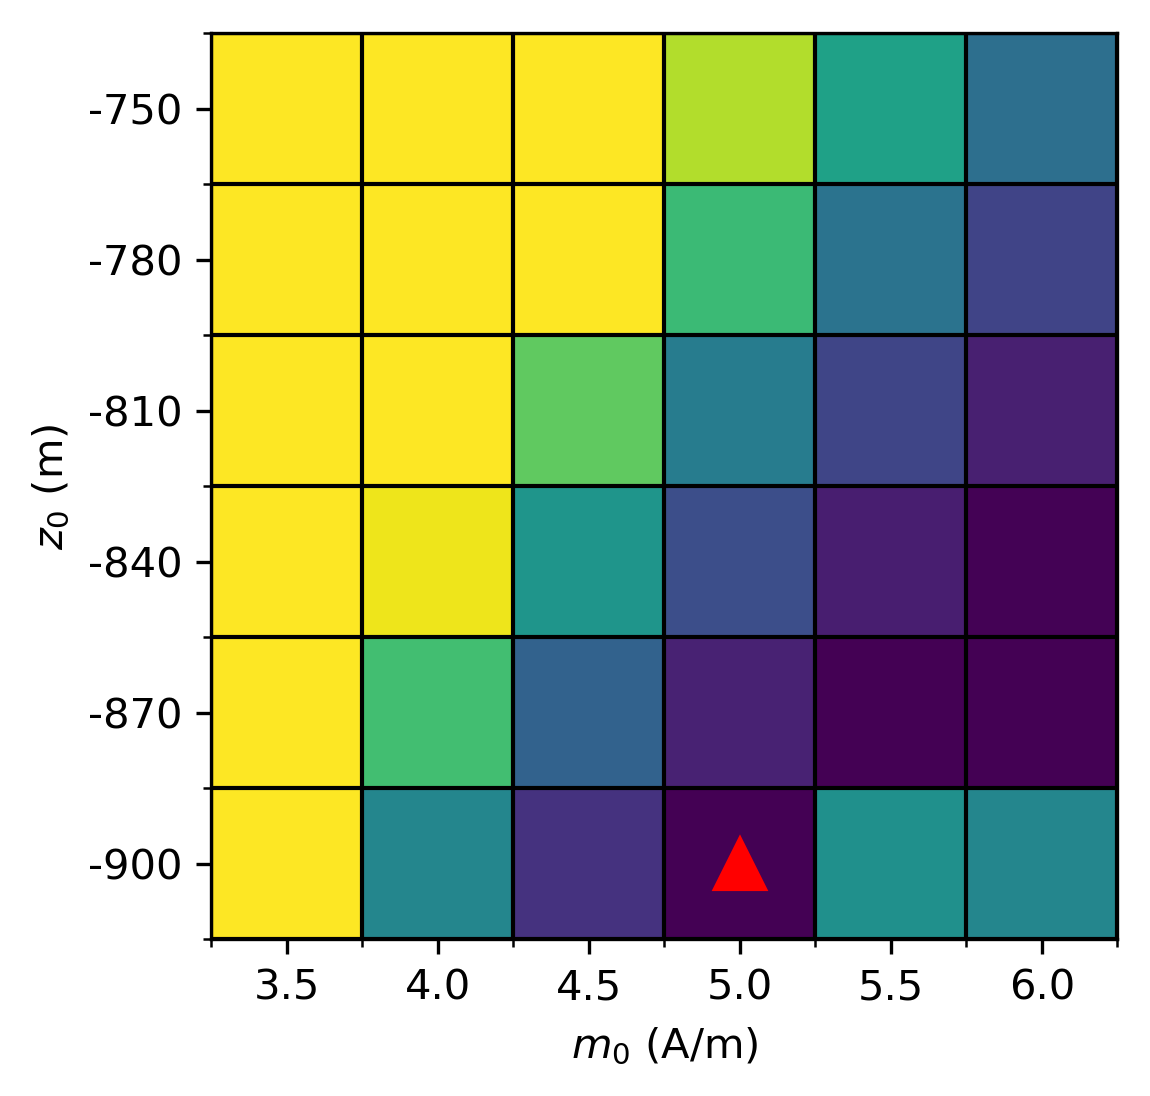
\includegraphics[scale=.75]{figures/anitapolis_goal_func_grid.png}
	\caption{Map of the objective function values due to the inverse solutions for the complex model. The range of the total-magnetization intensity varies from $m_0 = 3.5$ to $m_0=6$ A/m in a step of $0.6$ A/m and the range of the depth to the top  varies from $z_0=-900$ to $-750$ m in a step of $30$ m. Each square is a value of the goal function (eq. \ref{eq:gamma}) of a solution of the inverse problem for a pair of the total-magnetization intensity and the depth to the top of the source. These inversions were computed using the same cylinder as a initial approximation. The red triangle represents the lowest value of $ \Gamma(\mathbf{p}) $ for a pair of $m_0$ and $z_0$.
	}
	\label{fig:real_map}
\end{figure}

\begin{figure}
    \centering
    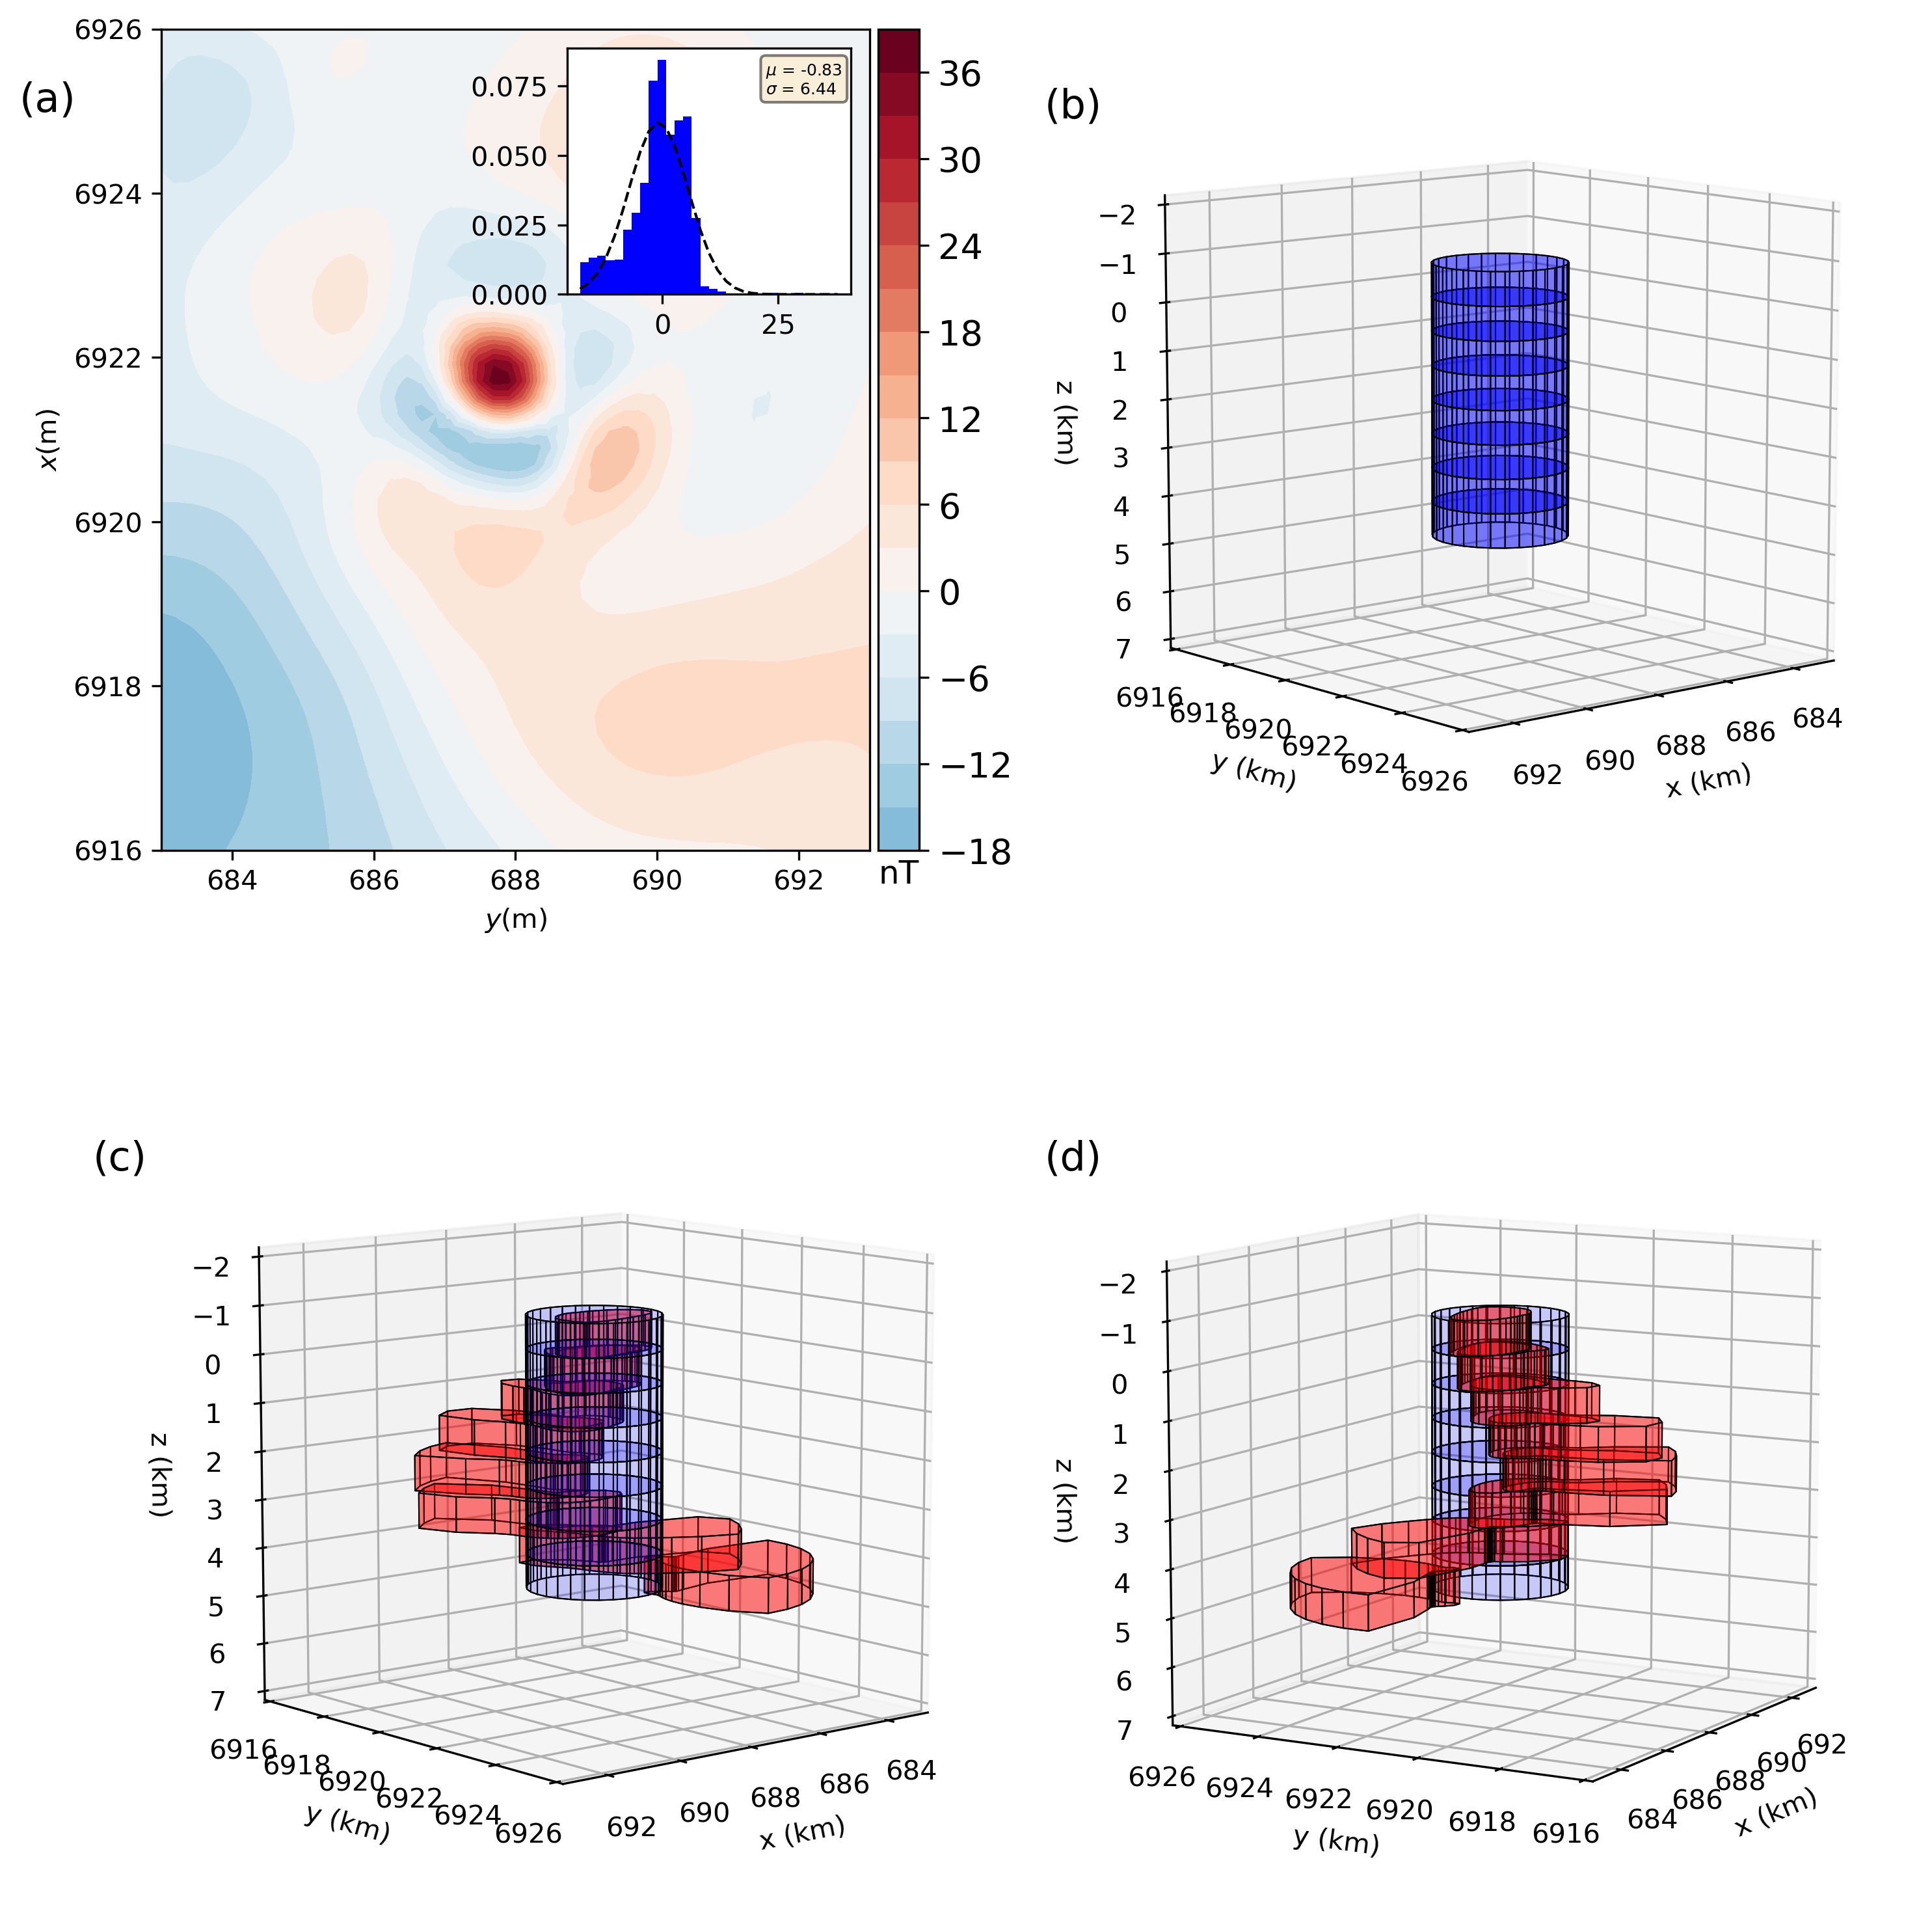
\includegraphics[scale=.5]{figures/anitapolis_results.png}
    \caption{Application to field data. (a) residual data given by the difference between the observed data (Fig. \ref{fig:real_data}a) and the predicted data (not shown). The blue prisms in (b) represent the initial approximate of the inversion. The red prisms in (c) and (d) represent the estimated model. 
}
    \label{fig:real_result}
\end{figure}